\documentclass[10pt, a4paper]{article}

\usepackage[english]{babel}
\usepackage{csquotes}
\usepackage[margin=0.75in]{geometry}
\usepackage{setspace}
\usepackage{amsmath}
\usepackage{graphicx}
\usepackage{booktabs}
\usepackage[style=apa, backend=biber]{biblatex}
\usepackage{algorithm}
\usepackage{algpseudocode}
\providecommand{\algorithmautorefname}{Algorithm}
\addbibresource{references.bib}
\usepackage{listings}
\usepackage{xcolor}
\usepackage{caption}
\usepackage{amssymb}
\captionsetup[algorithm]{font=tt, labelsep=colon}

\lstset{
    basicstyle=\ttfamily,
    columns=fullflexible,
    keepspaces=true,
    frame=single,
    breaklines=true
}

\usepackage[
    colorlinks=true,
    linkcolor=black,
    urlcolor=black,
    citecolor=black
]{hyperref}

\numberwithin{equation}{section}

\renewcommand{\familydefault}{\rmdefault}

\usepackage{titlesec}

% Section headings — small capitals
\titleformat{\section}
  {\normalfont\large\scshape}
  {\thesection.}
  {0.5em}
  {}

\titlespacing*{\section}
  {0pt}
  {2.0ex plus 0.5ex minus 0.2ex}
  {1.0ex plus 0.2ex}

% Subsection headings — normal
\titleformat{\subsection}
  {\normalfont\itshape\normalsize}
  {\thesubsection}
  {0.5em}
  {}

\titlespacing*{\subsection}
  {0pt}
  {1.5ex plus 0.3ex minus 0.2ex}
  {0.6ex plus 0.1ex}

% Subsubsection headings — italic
\titleformat{\subsubsection}
  {\normalfont\itshape\normalsize}
  {\thesubsubsection}
  {0.5em}
  {}

\titlespacing*{\subsubsection}
  {0pt}
  {1.2ex plus 0.3ex minus 0.2ex}
  {0.4ex plus 0.1ex}

\title{
    Particle Filter Methods\\[0.5em]
    \large\itshape Measuring Underlying Volatility of NZD/USD Exchange Rates
}

\author{Eneti Tofa}
\date{October 2026}

\begin{document}


\maketitle
\thispagestyle{empty}
\newpage
\thispagestyle{empty}
\null{}
\newpage
\setcounter{page}{1}

\onehalfspacing{}

\section{Introduction}
A dynamical system is defined as a process whose internal state evolves over time according to governing transition rules, typically driven by a combination of deterministic and stochastic equations \parencite{Sarkka2013}. While conventional time series analysis often focuses on directly observable variables, many research applications require the estimation of latent state variable. In these systems, the underlying drivers are latent (unobserved) and can only be inferred indirectly through noisy, sequentially arriving measurements \parencite{Durbin2012}. Within this framework, classical linear-Gaussian dynamical systems are particularly advantageous, as they admit exact analytical solutions. However, real-world problems frequently depart from these idealised systems and are often characterised by non-linearity, multiplicative shocks, or non-Gaussian distributions, rendering traditional analytical methods intractable and motivating the need for more advanced methods \parencite{Arulampalam2002}. 

The necessity of tracking hidden states has made the use of latent dynamical systems ubiquitous across different disciplines. In physics and engineering, these models are foundational to problems ranging from basic kinematics, radar target tracking, aerospace navigation, robotics, and signal processing \parencite{Gustafsson2002, Sarkka2013}. In econometrics, state-space methods are widely deployed to estimate unobserved macroeconomic states, including output gaps and time-varying parameters, as well as latent stochastic volatility \parencite{Kim1998, Durbin2012}. Furthermore, these probabilistic formulations have become standard in epidemiology and ecology for tracking latent infection rates and unobserved population dynamics \parencite{BUCKLAND2004157, Dukic01122012} 

\subsection{Problem Introduction}
Consider a recursive state estimation problem where the goal is to estimate a state vector \(h\). For a dynamical system, the objective more specifically is to track the hidden state sequence \(h_t\), where \(t \in \mathbb{N}\) is a discrete time step. As the state is hidden, it cannot be directly measured using conventional methods. In order to estimate the hidden state, (at least) two models are required \parencite{Arulampalam2002}
\begin{enumerate}
    \item A model that describes prior knowledge on the expected evolution of the state \(h_t\) through time (System Model).
    \item A model that relates measurements \(y_t\) to the state \(h_t\) (Measurement Model).
\end{enumerate}

For problems where the information of the system is updated with the arrival of new measurements and the models are avaliable in a probabilistic form, the Bayesian approach to estimation is inherently suited. Consequently, the state vector is treated as a random variable, with its uncertainty represented by a probability distribution. Bayes' theorem can then be implemented to refine the belief based on a prior and new measurements. The objective thus is to construct the posterior density function based on all the current information. Since the pdf constitutes all the known information about the system, it can be considered a complete solution to the estimation problem \parencite{Elfring2021,Arulampalam2002}. 

When inference is performed offline over a fixed dataset, batch Markov chain Monte Carlo (MCMC) methods are highly effective for sampling the full posterior. However, for online tracking where sequential estimates must be continuously generated upon the arrival of new measurements, batch MCMC becomes computationally intractable because it requires evaluating the entire data sequence at every time step \parencite{Andrieu2010}. In these scenarios, a recursive filter is appropriate. Recursive filters bypass the need to reprocess historical data by continuously updating the posterior filtering density using only the preceding state estimate and the most recent observation, thus rendering real-time inference computationally feasible \parencite{Akyildiz2020}. A recursive filter consists of two stages \parencite{Arulampalam2002}
\begin{enumerate}
    \item Prediction: The system model is used to project the previous posterior filtering density forward in time, yielding the predictive prior density.
    \item Update: The predictive prior density is updated with the latest measurement via Bayes' theorem to form the current posterior filtering density.
\end{enumerate}
In some situations, an analytical solution is achievable, however, when the system or measurement models are non-linear, or the noise processes are non-Gaussian, the integrals required for the optimal Bayesian solution become analytically intractable. In such a case, a particle filter is an advisable method for approximating the solution \parencite{Elfring2021}.

\subsection{Scope}
The aim of this report is to establish the theoretical foundations of particle filtering methods, and to apply these methods to a stochastic volatility model to evaluate their effectiveness. To achieve this, Section 2 formulates the Sequential Importance Sampling (SIS) framework, addresses the inherent challenge of particle degeneracy via resampling techniques, and formally defines the generic particle filter algorithm. Section 3 then specifies a canonical discrete-time stochastic volatility model and evaluates the empirical filtering results alongside residual diagnostics using daily NZD/USD log-returns from 2018 to 2026. Finally, Section 4 critically evaluates the strengths, structural limitations, and practical application domains of the particle filtering methodology.

\section{Particle Filter Method}
\subsection{Sequential Importance Sampling}
Sequential Importance Sampling is a Monte Carlo (MC) method for implementing a recursive Bayesian filter using MC simulations. The method has various names including bootstrap filtering, interacting particle approximations, and commonly, particle filters \parencite{Gordon1993NovelAT, Arulampalam2002}. The objective is to represent the pdf of the state variable with a set of random samples with corresponding weights. These samples and weights are then used to compute estimates. As the sample size tends to infinity, the approximation becomes equivalent to the real pdf, and thus the particle filter approaches the optimal Bayesian estimate \parencite{Arulampalam2002}.

For the purposes of this report, let \({\left\{h_{1:t}^{i}, w_t^{i}\right\}}_{i=1}^{N}\) denote a random measure that characterises the joint posterior pdf \(p(h_{1:t} | y_{1:t})\), where \({\left\{h_{1:t}^{i}, i = 1, \dots, N\right\}}\) is a set of support points representing the state trajectories with associated weights \({\left\{w_t^{i}, i = 1, \dots, N\right\}}\). The joint posterior density is approximated as
\begin{equation}
    p(h_{1:t} | y_{1:t}) \approx \sum_{i=1}^N w_t^{i} \delta(h_{1:t} - h_{1:t}^{i}),
\end{equation}
where \(w_t^{i}\) is the normalised weight of the \(i\)th particle. Based on the principle of importance sampling, this importance weight is defined as the ratio of the joint posterior density to a proposal density (known as the importance density), evaluated for the $i$th particle
\begin{equation}
    w_t^{i} \propto \frac{p(h_{1:t}^{i} |{} y_{1:t})}{q(h_{1:t}^{i} |{} y_{1:t})}.
\end{equation}

Following the approach of \textcite{Arulampalam2002}, under the required conditions (see Appendix A), the weights can be represented as
\begin{equation}
    w_t^{i} \propto w_{t-1}^{i} \frac{f(y_t | h_t^{i}) f(h_t^{i} | h_{t-1}^{i})}{q(h_t^{i} | h_{t-1}^{i}, y_t)}, \label{eq: SIS weight}
\end{equation}
and thus the posterior filtering density is approximated as
\begin{equation}
    p(h_t |{} y_{1:t}) \approx \sum_{i=1}^N w_t^{i} \delta(h_t - h_t^{i}). \label{eq: Posterior PDF Method}
\end{equation}

The SIS algorithm thus follows a recursive loop: As each new measurement \(y_t\) is received, the particles are propagated forward in time and their importance weights are updated. This process is formalised in \autoref{alg:sis}.

\begin{algorithm}[ht]
\caption{SIS Particle Filter}\label{alg:sis}
\begin{algorithmic}[1]
\ttfamily
\For{$i = 1,\dots,N$}
    \State{Draw $h_t^{i} \sim q(h_t | h_{t-1}^{i}, y_t)$}
    \State{Assign the particle a weight, \(w_t^{i}\), according to \autoref{eq: SIS weight}}
\EndFor{}
\end{algorithmic}
\end{algorithm}


\subsection{Resampling}

Over successive iterations, sequential Monte Carlo methods suffer from particle degeneracy, where the variance of the weights increases until a single particle dominates the distribution. There are several ways to mitigate this, however, this report focuses on resampling. The general goal is to eliminate particles with small weights and replace them with particles cloned from higher-weight particles. This means taking a random sample directly from the approximate discrete posterior pdf given by \autoref{eq: Posterior PDF Method}. 

To achieve this, a cumulative distribution function (CDF) of the normalised weights is constructed, and a new set of \(N\) particles is drawn from this distribution. Because a particle's importance weight dictates the width of its corresponding interval in the CDF, particles with large weights have a high probability of being drawn multiple times (cloned), while particles with negligible weights are more likely to be eliminated. Because the concentration of these newly drawn particles now perfectly represents the shape of the posterior distribution, the weights are reset to uniformity \(w_t^{i} = \frac{1}{N}\). Various algorithmic schemes exist to perform the draw such as multinomial, systematic, stratified or residual resampling \parencite{Douc2005,Elfring2021}.

In practice, carrying out resampling at every time step is computationally expensive and introduces unnecessary Monte Carlo variance into the estimates. Therefore, the Effective Sample Size (ESS) is monitored continuously to serve as a threshold for resampling. The ESS is approximated by (see \textcite{Kong1994SequentialIA})
\begin{equation}
    N_{eff} = \frac{1}{\sum_{i=1}^N {(w_t^{i})}^2}.\label{eq: ess}
\end{equation}
When \(N_{eff}\) falls below a predefined threshold \(N_T\), the algorithm performs the resampling step. 
In the following section, the generic particle filter algorithm (\autoref{alg:gpf}) is implemented.

\begin{algorithm}[ht]
\caption{Generic Particle Filter}\label{alg:gpf}
\begin{algorithmic}[1]
\ttfamily
\For{$i = 1,\dots,N$}
    \State{Draw $h_t^{i} \sim q(h_t | h_{t-1}^{i}, y_t)$}
    \State{Assign the particle an unnormalised weight, \(w_t^{i}\), according to \autoref{eq: SIS weight}}
\EndFor{}
\State{Calculate total weight: \(W = \sum_{i=1}^N w_t^{i}\)}
\For{$i = 1,\dots,N$}
    \State{Normalise: \(w_t^{i} = W^{-1} w_t^{i}\)}
\EndFor{}
\State{Calculate \(N_{eff}\) using \autoref{eq: ess}}
\If{\(N_{eff} < N_T\)}
    \State{Resample \(N\) particles using chosen method}
    \State{Reset weights: \(w_t^{i} = 1/N\) for all \(i = 1,\dots,N\)}
\EndIf{}
\end{algorithmic}
\end{algorithm}

\subsection{Other Particle Filters}
Extensions to the generic particle filter have been developed to address specific estimation challenges. For instance, the Sampling Importance Resampling (SIR) filter simplifies this architecture by explicitly defining the prior transition density as the importance proposal, an approach frequently utilised in non-linear target tracking \parencite{Arulampalam2002}. To improve efficiency when observations are highly informative, the Auxiliary Particle Filter introduces a predictive step prior to resampling \parencite{Pitt1999}. A Regularised Particle Filter mitigates sample depletion by resampling from a continuous kernel density approximation rather than a discrete measure \parencite{marti2011regularised}. There are numerous further forms of particle filters including hybrid approaches \parencite{Casarin2009, Elfring2021, Arulampalam2002}. Because these advanced algorithms are fundamentally specialised variations of the generic particle filter, a comprehensive analysis of each falls beyond the scope of this report, and the following example will utilise only the generic particle filter.

\section{Example}

Consider the recursive state estimation problem where one wishes to measure the underlying volatility of an exchange rate, $h_t$, based on observations of its daily log-returns, $y_t$. As the volatility is latent, and thus cannot be directly measured, the primary objective of this section is to use the methods previously discussed to estimate this hidden state. More specifically, the objective is to estimate the log volatility over time of the New Zealand Dollar to US Dollar (NZD/USD) exchange rate using empirical data.

\subsection{Model}
Stochastic volatility modeling relies heavily on Bayesian updating to track hidden state variables. The typical volatility model for regularly spaced data is formalised by the following system \parencite{Kim1998}
\begin{align}
    y_t &= \beta e^{h_t / 2} \epsilon_t, \quad \quad t \geq 1, \label{eq: measurement model} \\
    h_{t+1} &= \mu + \phi\left(h_t - \mu\right) + \sigma_\eta \eta_t, \label{eq: system model} \\
    h_1 &\sim \mathcal{N}\left(\mu, \frac{\sigma_\eta^2}{1 - \phi^2}\right),
\end{align}
where \(y_t\) is the return on holding the asset at time \(t\), \(h_t\) is the log volatility at time \(t\) which is assumed to follow a stationary process (\(|\phi| < 1\)) with \(h_1\) drawn from the stationary distribution, \(\epsilon_t\) and \(\eta_t\) are uncorrelated standard normal white noise shocks. The parameter \(\beta\) is the constant scaling factor representing the modal instantaneous volatility, \(\phi\) represents persistence in the volatility, and \(\sigma_\eta\) the volatility of the log-volatility \parencite{Kim1998}. In this scenario, \autoref{eq: measurement model} is the Measurement Model and \autoref{eq: system model} the System Model. As the objective is to estimate the underlying volatility at each time step, a sequential filter is preferred to MCMC methods.

To represent this system in a standard Bayesian framework, the conditional distributions and their corresponding probability density functions are defined. 

Because the measurement noise term $\epsilon_t$ is defined as an independent standard normal variable, the resulting conditional distribution is Gaussian. Conditional on the log volatility \(h_t\), the observation \(y_t\) thus follows a zero-mean Normal distribution with standard deviation corresponding to the coefficient on \(\epsilon_t\)
\begin{equation}
    y_t | h_t \sim \mathcal{N}\left(0, \beta^2 e^{h_t}\right),
\end{equation}
yielding the measurement density
\begin{equation}
    f(y_t | h_t) = \frac{1}{\sqrt{2\pi\beta^2 e^{h_t}}} \exp\left(-\frac{y_t^2}{2\beta^2 e^{h_t}}\right).
\end{equation}

For the prior, because the latent log-volatility $h_t$ follows a Markov process, its evolution is conditional solely on the previous state, $h_{t-1}$. As it is assumed that the log-volatility follows an AR (1) process in acordance with \textcite{Taylor1999}, and given the system noise term $\eta_t$ is an independent standard normal variable, the conditional transition distribution is strictly Gaussian. Therefore, the log volatility $h_t$ follows a Normal distribution centered at its deterministic autoregressive mean, $\mu + \phi (h_{t-1} - \mu)$, with a standard deviation given by the coefficient on the system noise $\eta_t$.

\begin{equation}
    h_t | h_{t-1} \sim \mathcal{N}\left(\mu + \phi(h_{t-1} - \mu), \sigma_\eta^2\right),
\end{equation}
which defines the state transition density
\begin{equation}
    f(h_t | h_{t-1}) = \frac{1}{\sqrt{2\pi\sigma_\eta^2}} \exp\left(-\frac{{\big(h_t - \mu - \phi(h_{t-1} - \mu)\big)}^2}{2\sigma_\eta^2}\right).
\end{equation}

The predictive prior density is obtained by integrating the state transition density over the posterior distribution from the previous time step via the Chapman-Kolmogorov equation \parencite{Arulampalam2002}
\begin{equation}
    p(h_t | y_{1:t-1}) = \int f(h_t | h_{t-1}) p(h_{t-1} | y_{1:t-1}) dh_{t-1}.
\end{equation}

By Bayes' theorem, the posterior filtering density is therefore given by

\begin{equation}
    p(h_t | y_{1:t}) = \frac{f(y_t | h_t) p(h_t | y_{1:t-1})}{\int f(y_t | h_t) p(h_t | y_{1:t-1}) dh_t}.
\end{equation}

Because the measurement density \(f(y_t | h_t)\) is highly non-linear with respect to the state \(h_t\), the denominator integral is analytically intractable. This precludes exact filtering and motivates the use of a particle filter to approximate the posterior.

\subsection{Importance density}
There are a plethora of choices for the importance density \(q(h_t^{i} | h_{t-1}^{i}, y_t)\), including the optimal importance density and local approximations via Extended or Unscented Kalman Filters \parencite{Elfring2021}. However, in this case, the most convenient choice is simply the prior, \(f(h_t | h_{t-1})\). Subsequently, the denominator cancels with the prior in the numerator in \autoref{eq: SIS weight}. The weight update equation thus collapses to the likelihood
\begin{equation}
    w_t^{i} \propto w_{t-1}^{i} f(y_t | h_t^{i}).
\end{equation}
The assumptions required for this are weak and all satisfied by the model, mainly: (1) one can sample directly from the prior, and (2) the likelihood \(f(y_t | h_t)\) can be evaluated pointwise \parencite{Arulampalam2002}.

\subsection{Data and Implementation}
The example uses daily NZD/USD from 2018 to 2026 exchange rate data published by the Reserve Bank of New Zealand \parencite{rbnz2026}. Prior to sequential analysis, the raw exchange rates, \(P_t\), were transformed into daily log-returns to construct the observations

\begin{equation}
    y_t = 100 \times \ln(P_t / P_{t-1}).
\end{equation}


The stochastic volatility model was estimated using the generic particle filter outlined in \autoref{alg:gpf}. The simulation was implemented in R utilising \(N = 1000\) particles. To combat particle degeneracy, the effective sample size threshold was set to \(N_T = N/2 = 500\). Whenever \(N_{eff}\) dropped below this limit, a multinomial resampling scheme was executed to replenish the particle pool.

Finally, to extract a practical point estimate of the latent volatility at any given time step \(t\), the expected value of the posterior filtering density was approximated via the weighted sum of the particles
\begin{equation}
    \hat{h}_t = \sum_{i=1}^N w_t^{i} h_t^{i}.
\end{equation}

\begin{algorithm}[ht]
\caption{Stochastic Volatility Particle Filter}\label{alg:svpf}
\begin{algorithmic}[1]
\ttfamily
\State{Initialize at \(t=1\):}
\For{\(i = 1,\dots,N\)}
    \State{Draw \(h_1^{i} \sim \mathcal{N}\left(\mu, \frac{\sigma_\eta^2}{1 - \phi^2}\right)\)}
    \State{Assign initial weight \(w_1^{i} = 1/N\)}
\EndFor{}
\State{Calculate initial point estimate: \(\hat{h}_1 = \sum_{i=1}^N w_1^{i} h_1^{i}\)}
\For{\(t = 2,\dots,T\)}
    \For{\(i = 1,\dots,N\)}
        \State{Draw \(h_t^{i} \sim \mathcal{N}\left(\mu + \phi(h_{t-1}^{i} - \mu), \sigma_\eta^2\right)\)}
        \State{Evaluate measurement density: \(f(y_t | h_t^{i}) = \frac{1}{\sqrt{2\pi\beta^2 \exp(h_t^{i})}} \exp\left(-\frac{y_t^2}{2\beta^2 \exp(h_t^{i})}\right)\)}
        \State{Update unnormalised weight: \(w_t^{i} = w_{t-1}^{i} f(y_t | h_t^{i})\)}
    \EndFor{}
    \State{Calculate total weight: \(W = \sum_{i=1}^N w_t^{i}\)}
    \For{\(i = 1,\dots,N\)}
        \State{Normalise weights: \(w_t^{i} = W^{-1} w_t^{i}\)}
    \EndFor{}
    \State{Calculate \(N_{eff} = {\left(\sum_{i=1}^N {(w_t^{i})}^2\right)}^{-1}\)}
    \If{\(N_{eff} < N/2\)}
        \State{Resample \(N\) particles using multinomial resampling}
        \State{Reset weights: \(w_t^{i} = 1/N\) for all \(i = 1,\dots,N\)}
    \EndIf{}
    \State{Calculate point estimate: \(\hat{h}_t = \sum_{i=1}^N w_t^{i} h_t^{i}\)}
\EndFor{}
\end{algorithmic}
\end{algorithm}

The parameters governing the system and measurement equations are calibrated to fit standard empirical estimates for daily exchange rate log-returns. For identifiability reasons, the scaling factor is fixed at \(\beta = 1\). The persistence parameter is set to \(\phi = 0.93\), while the state noise standard deviation is set to \(\sigma_\eta = 0.2\). Finally, the long-run mean is set to \(\mu = -1\). All parameters are adjusted to fit the NZD/USD exchange rate data in accordance with the ranges found in the literature \parencite{Kim1998}.

\subsection{Results}

The particle filter was applied to the daily NZD/USD log-returns. \autoref{fig:returns} displays the observed daily log-returns \(y_t\), highlighting distinct periods of volatility clustering, most notably the significant shock in early 2020 corresponding to the onset of the COVID-19 pandemic. \autoref{fig:volatility} demonstrates the particle filter's estimate of the latent log-volatility state, \(\hat{h}_t\). The filter closely tracks the sudden spikes in market variance while exhibiting the mean-reverting behavior expected from the system model.

The degeneracy of the generic particle filter is monitored in \autoref{fig:neff}. The effective sample size, \(N_{eff}\), frequently drops below the predefined threshold of \(N/2 = 500\), triggering the multinomial resampling step. This confirms that the algorithm is actively mitigating particle degeneracy as expected, successfully removing low-weight trajectories and cloning high-likelihood particles to maintain a representative approximation of the posterior filtering density. Notably, the largest degeneracies tend to occur around the shocks, indicating the importance of resampling for these types of volatility problems.

To evaluate the performance of the model, \autoref{fig:comparison} contrasts the instantaneous variance implied by the particle filter against a naive 30-day rolling variance. The particle filter reacts almost instantaneously to sudden market shocks where the 30-day rolling variance takes notably more time steps to reach peak volatility. Furthermore, the particle filter returns to stability quicker than the rolling variance. Specifically, it avoids the issue where an extreme observation inflates the estimated volatility for the following time steps.

Finally, the adequacy of the method is evaluated by examining the residuals. Given the measurement model and the constraint \(\beta = 1\), the empirical residuals are extracted via 
\begin{equation}
    u_t = y_t / \exp(\hat{h}_t / 2).
\end{equation} 
If the filter adequately captures the volatility clustering present in the raw data, the squared standardised residuals, \(u_t^2\), should behave as independent white noise. \autoref{fig:acf} plots the autocorrelation function (ACF) of \(u_t^2\). The vast majority of lags fall within the 95\% confidence bounds, indicating that the systematic volatility dynamics have been successfully absorbed into the hidden state \(h_t\).


\begin{figure}[htbp]
    \centering
    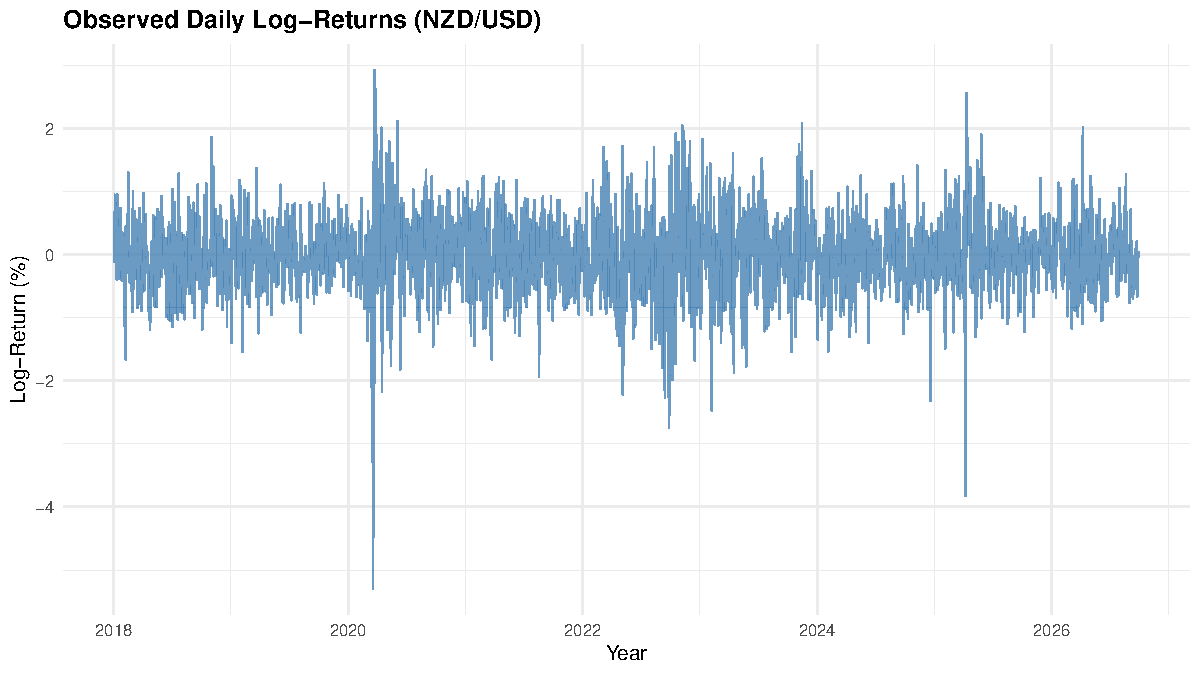
\includegraphics[width=0.9\textwidth]{figures/1_log_returns.pdf}
    \caption{Daily log-returns (\(y_t\)) of the NZD/USD exchange rate.}\label{fig:returns}
\end{figure}

\begin{figure}[htbp]
    \centering
    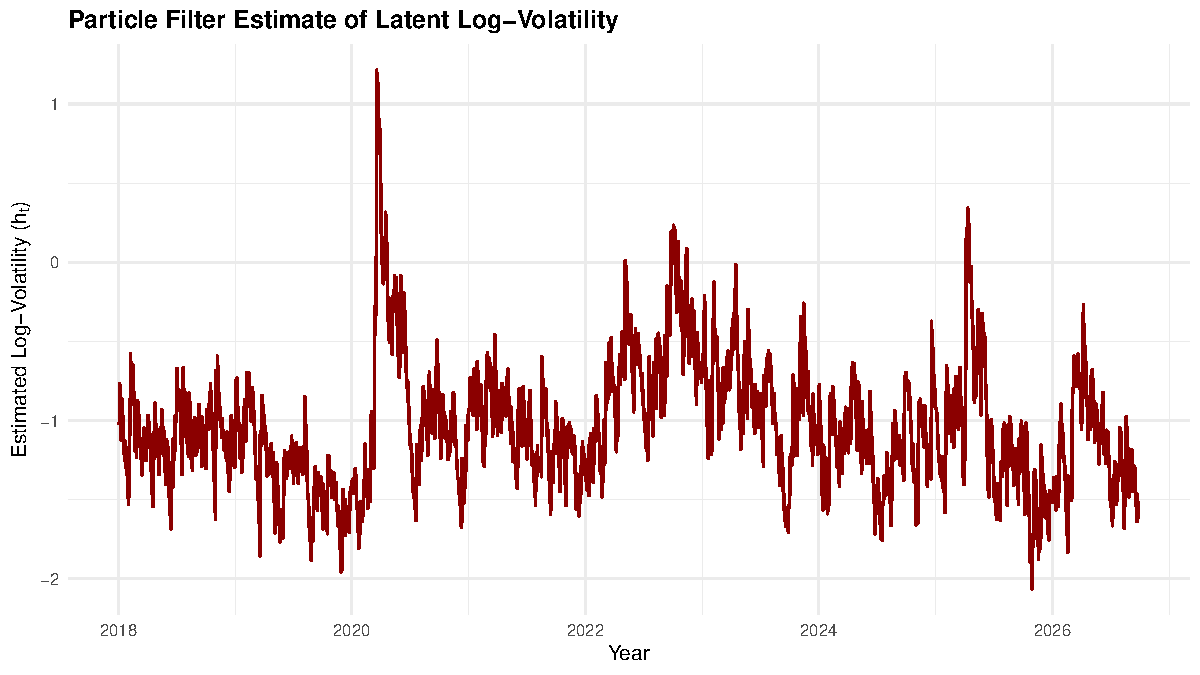
\includegraphics[width=0.9\textwidth]{figures/2_filtered_volatility.pdf}
    \caption{Particle filter estimate of the latent log-volatility state (\(h_t\)).}\label{fig:volatility}
\end{figure}

\begin{figure}[htbp]
    \centering
    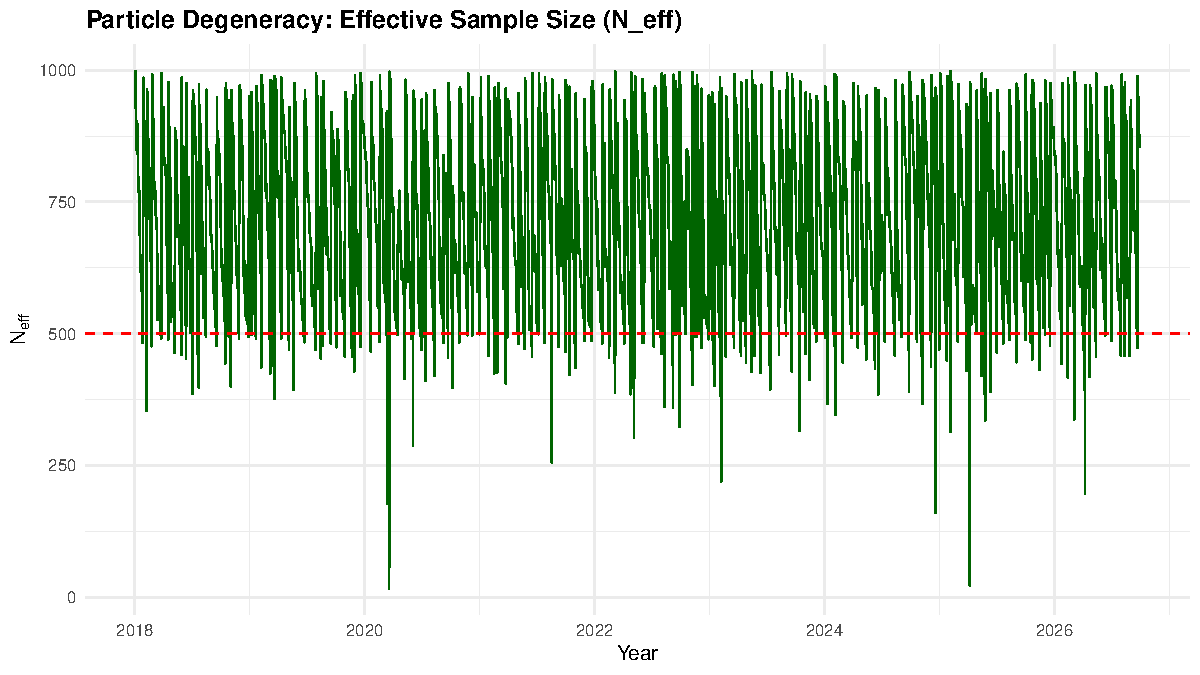
\includegraphics[width=0.9\textwidth]{figures/3_effective_sample_size.pdf}
    \caption{Effective Sample Size (\(N_{eff}\)) diagnostic tracking particle degeneracy. The horizontal dashed red line indicates the algorithmic safety net at \(N/2 = 500\).}\label{fig:neff}
\end{figure}

\begin{figure}[htbp]
    \centering
    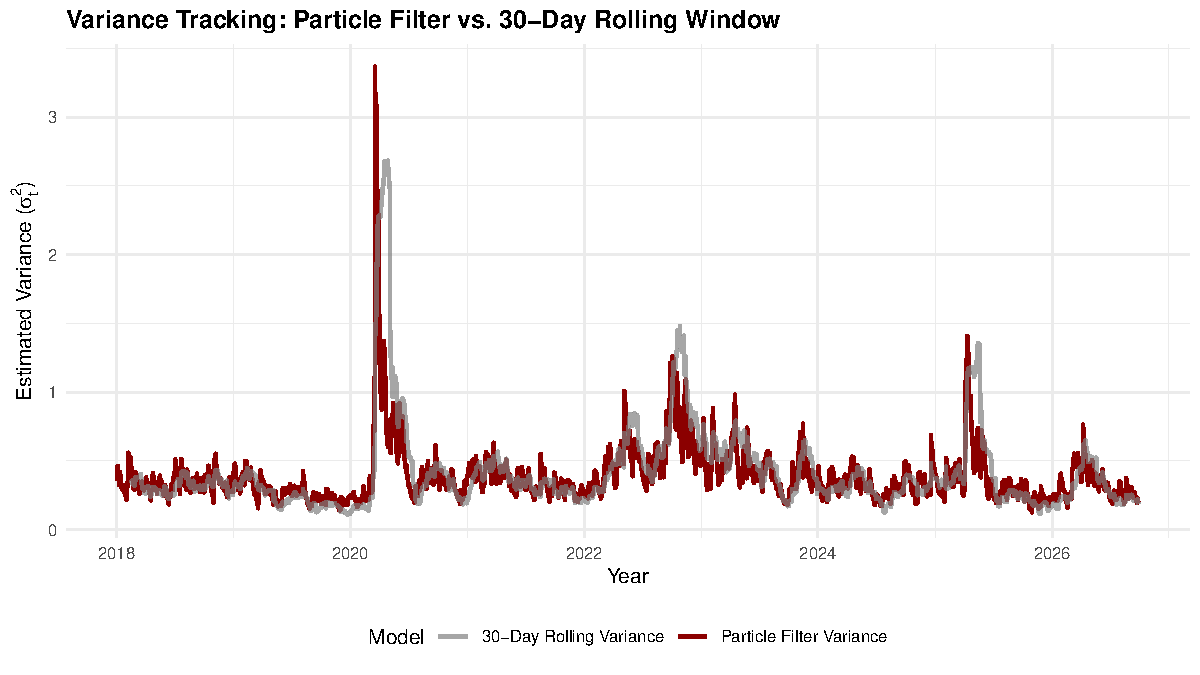
\includegraphics[width=0.9\textwidth]{figures/4_variance_comparison.pdf}
    \caption{Comparison of estimated variance (\(\sigma_t^2\)) between the stochastic volatility particle filter and a naive 30-day rolling window.}\label{fig:comparison}
\end{figure}

\begin{figure}[htbp]
    \centering
    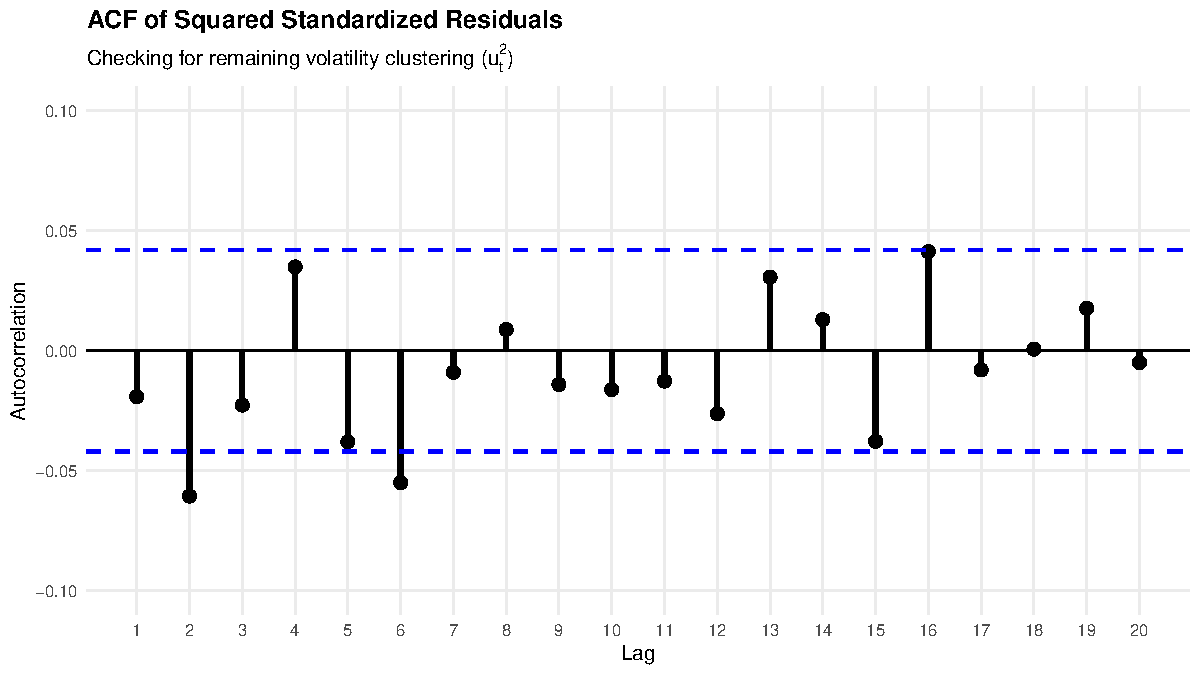
\includegraphics[width=0.9\textwidth]{figures/5_acf_residuals.pdf}
    \caption{Autocorrelation function (ACF) of the squared standardized residuals (\(u_t^2\)).}\label{fig:acf}
\end{figure}

\section{Discussion}

The application of the generic particle filter successfully extracted the latent stochastic volatility of the NZD/USD exchange rate. By recursively approximating the posterior filtering density, the algorithm avoided the analytically intractable integrals introduced by the non-linear measurement equation. As demonstrated by the outputs, the method's primary strength lies in its dynamic adaptability. The filter tracked sudden market shocks instantaneously, outperforming the 30-day rolling variance. Furthermore, the framework effectively absorbed the systematic volatility clustering inherent to the data.

These findings highlight the utility of the particle filter for real-time sequential inference. Because the algorithm continuously updates the probability distribution of the hidden state using only the preceding posterior and the latest observation, it requires minimal memory and fixed computational time per step. Consequently, this methodology is highly recommended for online state estimation problems. Such problems include positioning, dynamic navigation, and non-linear target tracking \parencite{Arulampalam2002, Gustafsson2010, Gustafsson2002}. Additionally, as shown in this work, it provides a computationally tractable framework for the sequential filtering of stochastic volatility where the computational cost of batch processing is prohibitive \parencite{Kim1998}.

Despite these advantages, the implemented methodology possesses several limitations. A primary weakness of the generic filter is its reliance on the prior transition density as the importance proposal. Because this unguided mechanism ignores current observations, extreme observations, such as the early 2020 pandemic shock, cause rapid particle degeneracy. This forces the algorithm to rely heavily on multinomial resampling, which discards information and introduces Monte Carlo variance. Furthermore, the implemented filter relied on pre-calibrated static parameters (\(\mu\), \(\phi\), \(\sigma_\eta\)) rather than jointly estimating them from the data. Therefore, this framework is not recommended for retrospective analysis where exact parameter estimation is the objective. In such scenarios, batch Markov chain Monte Carlo (MCMC) methods are superior. Additionally, the generic particle filter should be avoided in highly multidimensional volatility models, as the particle volume required to prevent degeneracy scales exponentially with the state dimension.

\newpage
\singlespacing{}

\section*{Code Accessibility}
Code used for simulations can be found at \url{https://github.com/EnetiTofa/Fiscal-Taylor-Rule}.

\printbibliography{}

\end{document}